\section{Gary}

\begin{center}
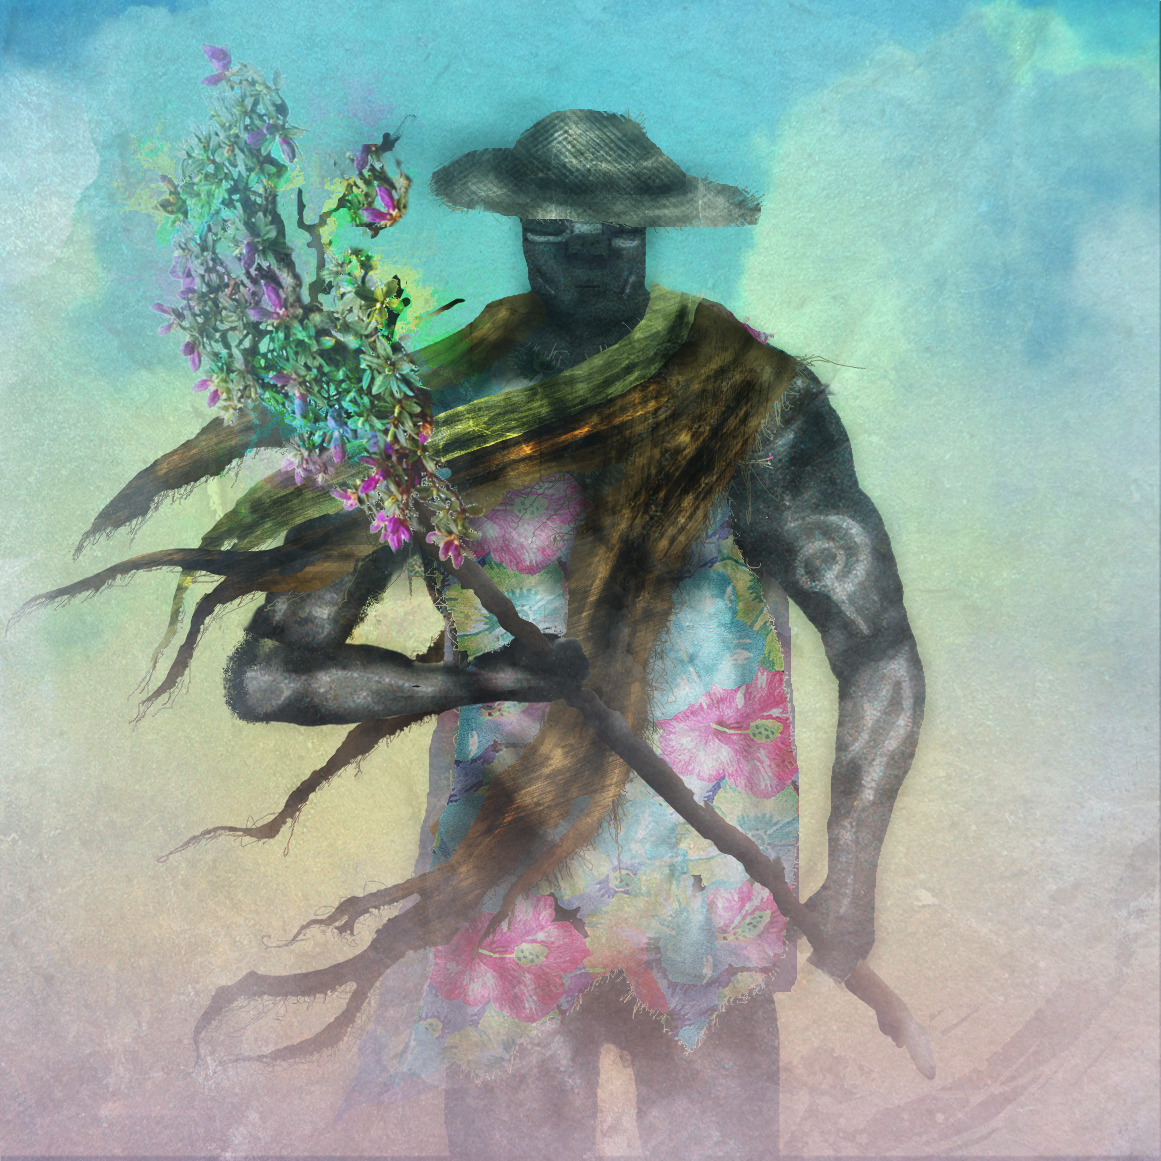
\includegraphics[width=80mm]{./content/img/gary.png}
\begin{figure}[h]
\end{figure}
\end{center}

\subsection*{Details}

\noindent

Race: 	Stone Man \\
Class: 	Police \\
Age: 	8,000,000 \\
Status: Sleeping

\subsubsection{Background}

Gary was an ancient stone elemental, a living statue who had stood motionless for millennia before being awakened by the party during their quest for the Gulan bush.  After consuming a magical biscuit, Gary discovered the joy of eating, breathing, and existing, and immediately became one of the group's most beloved and formidable companions.

Gary's origins stretch back to the dawn of the world.  Long before the Sundering, the Ancients built a standing stone, to protect.  He recalled stories of figures like Jason Derulo, ``who was sat on by a thing and killed thousands of years ago'', though his knowledge of The Ancients was limited, ``he's just a rock''.

\subsubsection{Personality and Traits}

Gary was the group's moral heart.  A pacifist by nature, he fought only when necessary and always sought to talk before striking.  His philosophy was simple and profound, he believed in the goodness of all creatures and the power of second chances.  He once convinced a group of enemies to rethink their lives and ``settle down, get a job, contribute productively to society''.

In combat, Gary wielded a magical flowering branch that could emit rainbows and glitter, put enemies to sleep, and deliver devastating ``glitter bonks''.  He joined the Hope's Rest police force as Officer Djago, earning a double-sized truncheon and a half-orc partner.  He drew three-panel comics featuring the popular cat ``Triplicate'' instead of signatures.

Gary developed several unexpected habits during his time with the group: an oxygen addiction (courtesy of Pilch), a brief chemical dependency on Gabrin Kokaine, and a passion for eating that bordered on the problematic, he once ate all the bake sale pies overnight.

\subsubsection{Relationships}

Gary cared deeply for every member of the group, often healing fallen enemies and allies alike.  His bond with Kolo was particularly strong, the two shared philosophical conversations about business, life, and the nature of goodness, even if Kolo kept trying to get him addicted to various substances.

Delilah attempted to flirt with Gary on multiple occasions, to no avail.  Gary's expressionless stone visage made it difficult to read his emotions, but those who knew him could see the depth of feeling behind those ancient eyes.

\subsubsection{Gary's Story}

Gary's defining moment came during the battle at the Tikituk Temple in the jungles of South Africa.  Facing overwhelming odds, Gary sacrificed himself to protect Kolo, standing tall and proud as a horde of TikkiTucks hacked him down piece by piece, transforming into a tree in his final moments.  Lazarus later confirmed that Gary would regenerate, but it would take several hundred years.

The party honoured Gary by naming their newly acquired airship after him, and by founding the Gary Guild, ``Garys Against Religion, Yo'', in Hope's Rest.  The guild's logo, drawn by Gary himself before his death, became a universal hit.  His legacy lived on in everything the group built: the guild, the airship, and the simple philosophy that people should be kind to each other.  In the group's absence, the Gary Guild was taken over by Garbigail, a woman who had survived poisoning, beaten chicken disease, and spoken to Gary in a vision, transforming it into a pseudo-religious peace movement.  When the time came for the final battle against the Church, the Garys answered the call, suffering heavy casualties at the Battle of Hope's Rest in service of the ideals their founder had lived and died for.

\begin{DndSidebar}{Gary's Philosophy}
``EATING IS GOOD!'', Gary, upon trying his first biscuit.

``It is impossible to have a cake and also eat a cake.'', Gary, on the nature of the universe.

``When I set my mind on a perp, there's nothing that's gonna get in my way\ldots\ except CORN!'', Officer Djago, lost in a cornfield.
\end{DndSidebar}


\begin{center}
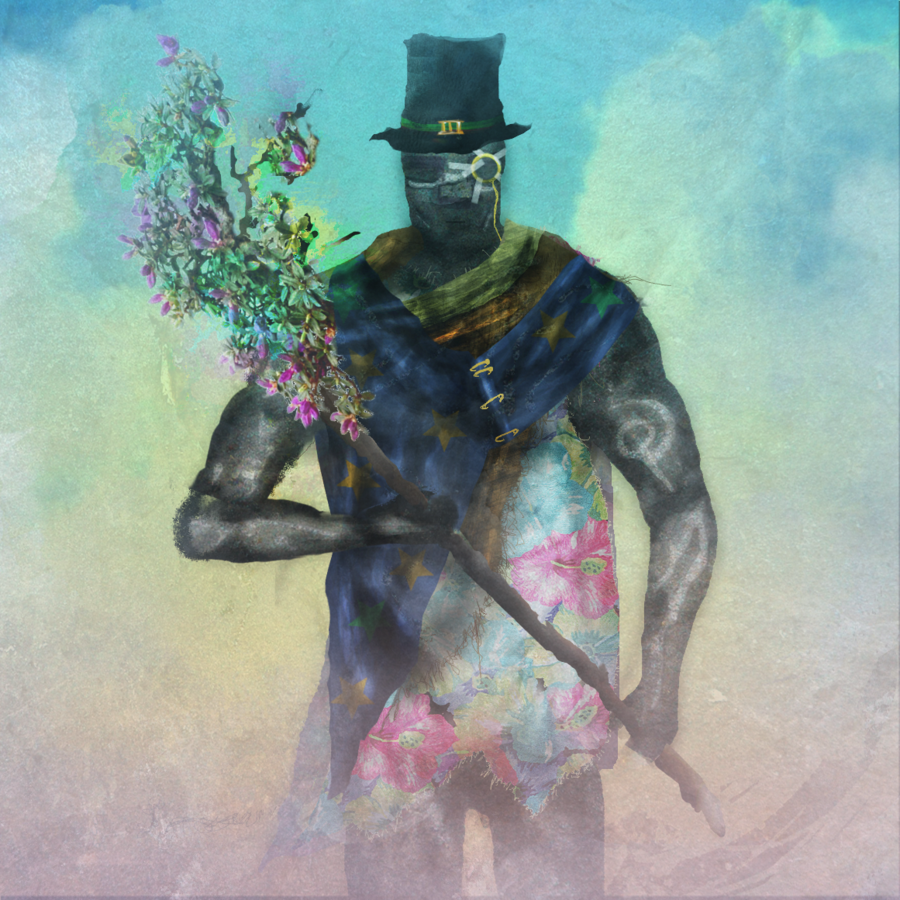
\includegraphics[width=80mm]{./content/img/reddit/officerDjago.png}\\
\textit{Jago, you know, just a guy about town, who does stuff}
\end{center}

\begin{center}
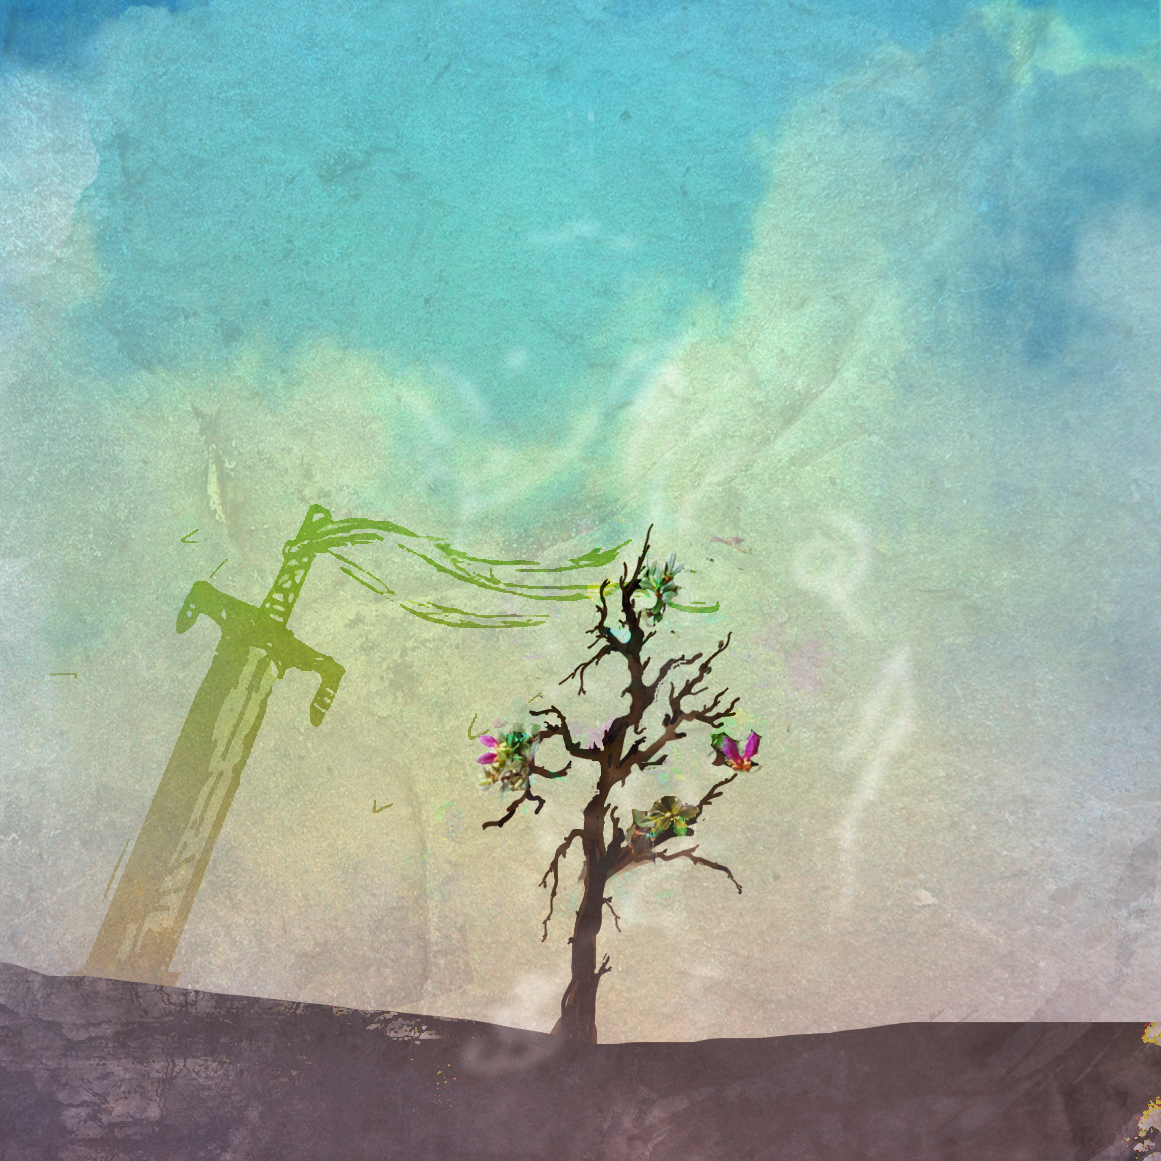
\includegraphics[width=80mm]{./content/img/garygrave.png}
\begin{figure}[h]
\end{figure}
\end{center}

\clearpage
